\documentclass[10pt,a4paper,portrait]{report}
\title{Annual Report}
\author{James Rogers}
\date{\today}

\usepackage{../format}
\usepackage{../commands}

\newcommand{\tabitem}{~~\llap{\textbullet}~~}

\addbibresource{../library.bib}

\begin{document}
\maketitle

\chapter{Introduction}
\section{Overview}\label{sec:introduction:overview}
A thin film is a layer of material that is applied to the surface of an object -- commonly referred to as the substrate -- to coat it. Typically a thin film
is less than several microns thick, though there is no universal agreed upon standard.
Thin film coatings find use in a wide range of industries and applications, ranging from hard mechanical coatings to reduce wear on an object, tribo-electrical coatings to capture wasted mechanical energy in the environment, or stacks of patterned coatings, which form the building blocks of modern micro-electronics, or optical coatings. \newline

\noindent
There are a variety of methods available to manufacture optical coatings, however, they are all types of \emph{additive} manufacturing, meaning that the films are grown;
This process is properly referred to as \emph{deposition}.
Deposition methods fall into one of two categories, physical vapour deposition (PVD) in which source material is converted into a vapour phase that condenses on the substrate, or chemical vapour deposition (CVD) where precursor species are introduced into a reaction vessel resulting in chemical reaction between them, forming coating material.
PVD can be further broken down into two sub-types of deposition: evaporation and sputtering.
In evaporation, the source material -- referred to as evaporant -- is heated so that it forms the vapour phase necessary to coat the substrate.
In sputtering the source material -- called target material -- is exposed to a plasma (typically argon);
The high energy ions impinge upon the surface of the target, causing atoms to eject -- or sputter -- from the target, thus forming a vapour phase. Different methods offer different advantages and disadvantages which have to be carefully considered when planning to deposit an optical coating.
For example, electron beam (e-beam) evaporation, has a very high rate of deposition ($\sim$nm/s), however can often result in porous films that are susceptible to index drift;
Magnetron sputtering on the other hand results in denser films, but at the cost of deposition rate ($\sim$\AA/s).\newline


\noindent
Optical coatings are useful because they allow us to manipulate the way in which light interacts with an optical interface.
Often, this can be altering the transmittance or reflectance of light at a single wavelength, or range of wavelengths in more complicated coatings;
Properties such as absorbance, phase of reflection/transmission, or 
polarisation are also highly desirable to control.
Common everyday applications of optical coatings include: anti-reflection coatings for spectacles, display devices, and scientific instruments, conductive transparent coatings for touch screens, demultiplexers for fibre optic communications, and many more.\newline

\noindent
When one designs an optical coating, there are two parameters for each layer that must be carefully considered.
The physical thickness of the layer, and  it's complex refractive index, which are denoted as $d$ and $n$ respectively.
The spectral properties of the coating are solely dependent on these set of parameters, in addition to the index of the ambient medium $n_0$, and that of the substrate $n_s$ \footnote{Only when one considers the multilayer in terms of an ideal model, further explanation will be provided in section}.
Often we find that variations in $n$ and $d$ in each layer can alter the spectral properties of the filter in an undesirable way, or even destroy them completely.
Thus it is necessary to be able to control them so that the deposition process is accurate and reliable. \newline

The earliest deposition systems achieved control by simply 


\section{Thin Film Optics}
\label{sec:thin film optics}

\subsection{First Principles}

\begin{equation}
\begin{aligned}
\nabla \cdot E &= \varepsilon^{-1}_{0}\rho &
\nabla \cdot B &= 0 \\
\nabla \times E &= -\frac{\partial B}{\partial t} &
\nabla \times B &= \mu_0 \left( J + \varepsilon_0 \frac{\partial E}{\partial t} \right)
\end{aligned}
\end{equation}

\noindent Any given material can be described by a dielectric function 
\begin{equation}
\epsilon(\omega) = \epsilon^{\prime} (\omega) + i \epsilon^{\prime\prime} (\omega), \;\; i = \sqrt{-1}
\end{equation}
where $\epsilon^{\prime}$ and $\epsilon^{\prime\prime}$ are the real and imaginary components of the function.
From the dielectric function we can compute the refractive index which is given as 
\begin{equation}
n = \sqrt{\mu_r \epsilon_r} = \frac{c_g}{v_g}
\end{equation}
for dielectric media, we set $\mu_r = 1$. $c_g$ and $v_g$ are the group velocities of light in vacuum and media respectively.

\subsection{Simple Dielectric Interface}\label{sec:simple-dielectric-interface}

A fundamental mathematical construction in optics is the `simple dielectric interface'; The interface is composed of two semi-infinite half spaces, which are infinite in the $xy$ plane, but not on the $z$ axis.
Each half space have a unique refractive index. The incident medium ($z<0$) has a refractive index of $n_1$, and the emergent ($z>0$) $n_2$. 
If we consider a monochromatic plane wave that impinges upon the interface, then the system can be reduced to a single axis $z$, assuming that the media are isotropic and homogeneous. The wave has an angle of incidence $\theta_1$, and $\theta_2$ in the emergent. A schematic of this setup is provided below.

\begin{figure}[H]
\begin{center}
\centering
\def\svgwidth{3in}
\input{simple-dielectric-interface.pdf_tex}
\end{center}
\label{simple-dielectric-interface}
\caption{A simple optical interface bounded by the two half-spaces $n_1$ and $n_2$, which illustrates the law of reflection $\theta_i=\theta_r$ and refraction, $\theta_1\neq\theta_2$ if $n_1 \neq n_2$, (Eq. \ref{eq:snells law})}
\end{figure}

At the interface some portion of the light will reflect away from the interface, and some will transmit through it.
The amplitudes of the reflected and transmitted waves are described by the Fresnel equations
The reflection coefficients for TE and TM polarised light are
\begin{align}
\label{fresnel-reflectance-coeff}
r_{TE} &= \frac{ n_1 \cos \theta_1 - n_2 \cos \theta_2}{n_1 \cos \theta_1 + n_2 \cos \theta_2} &
r_{TM} &= \frac{ n_1 \cos \theta_2 - n_2 \cos \theta_1 }{ n_1 \cos \theta_2 + n_2 \cos \theta_1} 
\end{align}
and the transmission coefficients are
\begin{align}
\label{fresnel-transmission-coeff}
t_{TE} &= \frac{ 2 n_1 \cos \theta_1 }{n_1 \cos \theta_1 + n_2 \cos \theta_2} &
t_{TM} &= \frac{ 2 n_1 \cos \theta_1 }{ n_1 \cos \theta_2 + n_2 \cos \theta_1}
\end{align}

\noindent
Using Snell's law we can calculate $\theta_2$
\begin{equation}\label{eq:snells law}
n_1 \sin \theta_1 = n_2 \sin \theta_2 \notag
\end{equation}
\begin{equation}
\theta_2 = \arcsin \left( \frac{n_1 \sin \theta_1 }{ n_2 } \right)
\end{equation}

\noindent
The power transmitted and reflected (which herein are solely referred to as transmittance and reflectance) at the interface can be calculated as follows

\begin{align}\label{eq:power-equations}
R &= |r|^2 &
T &= |t|^2
\begin{cases}
\dfrac{\Re \left( n_2 \cos\theta_2 \right)}{\Re \left( n_1 \cos\theta_1  \right)} & \mbox{for TE polarisation}\\[5mm]
\dfrac{\Re \left( n_2 \cos\theta_2^* \right)}{\Re \left( n_1 \cos\theta_1^* \right)} & \mbox{for TM polarisation}
\end{cases}
\end{align}

\subsection{Multilayer Thin Films}
As stated in Sec. \ref{sec:introduction:introduction to thin film optics} the properties of a multilayer stack can be described fully in terms of $n$ and $d$ for each layer, as well as the refractive indices of the incident and emergent media.
This assumes that every medium is isotropic, homogeneous, linear and infinite in the $xy$ plane.
If one makes such an assumption, then the stack can be modelled using the transfer-matrix-method (TMM). 
TMM was developed by Abel\`es \cite{abeles_sur_1948} \cite{abeles_theorie_1950} as an extension of Fresnel theory to account for the interference effects that occur within each layer.
The transfer matrix $\mathbf{M}$ relates the electric field amplitudes on each side of the multilayer structure to one another in the following manner.

\begin{equation}\label{eq:transfer-matrix-definition}
\begin{bmatrix}
  E^+\left( z_0 - \delta \right) \\
  E^-\left( z_0 - \delta \right)
\end{bmatrix} =
\mathbf{M}
\begin{bmatrix}
  E^+\left( z_k + \delta \right) \\
  E^-\left( z_k + \delta \right)
\end{bmatrix}
\end{equation}

\noindent
Where $E^+$ and $E^-$ are the forwards and backwards propagating components of the electric field, $z_0$ interface at the start of the stack, $z_k$ is the interface at the end of the stack, and $\delta \rightarrow 0$.
A schematic of this is provided below.

\vspace*{3mm}
\begin{figure}[H]
\label{multilayer-stack-interfaces}
\begin{center}
\centering
\def\svgwidth{4in}
\input{multi-layer-interfaces.pdf_tex}
\end{center}
\vspace*{-5mm}
\caption{Representation of a multilayer film stack with $k$ layers. The dashed lines represent the limit as one approaches $z_0$ from the left, or $z_k$ from the right}
\end{figure}%

\noindent
To calculate the transfer matrix, the characteristic matrix of a layer must first be introduced, which has the form

\begin{equation}
\label{eq:characteristic-matrix}
\mathbf{C} = 
\begin{bmatrix}
  \cos\phi         & i \sin \phi / N \\
  i \sin \phi \, N & \cos\phi
\end{bmatrix}
\end{equation}

\noindent
Where $\phi$ is the angular phase thickness of the layer, a measurement of the number of radians of a wave between the two interfaces of a layer for some wavelength $\lambda$.
$N$ is the effective index of the layer, which is adjustment made to account for polarisation at non-normal incidence. Formulae for $\phi$ and $N$ are given below; $n$, $d$, and $\theta$ have their usual meanings

\begin{equation}\label{angular-phase-thickness}
\phi = \frac{2\pi}{\lambda} nd \cos\theta
\end{equation}

\begin{equation}\label{effective-index}
N = 
\begin{cases}
  n\left(\cos\theta\right)^{-1} & \mbox{for TE polarisation} \\
  n\cos\theta      & \mbox{for TM polarisation}
\end{cases}
\end{equation}

\noindent
The characteristic matrix relates the $E$ and normalised $H$ fields at the interfaces $z_i$ and $z_{i+1}$ in the following manner
\begin{equation}
\label{eq:characteristic-matrix-fields}
\begin{bmatrix}
  E\left(z_i\right) \\
  Z_0 H \left( z_i \right)
\end{bmatrix} =
\mathbf{C}
\begin{bmatrix}
  E \left(z_{i+1}\right) \\
  Z_0 H \left(z_{i+1}\right) 
\end{bmatrix}
\end{equation}

\noindent
One can see that the relationship in Eq. \ref{eq:characteristic-matrix-fields} is recursive in nature. 
To compute a $\mathbf{C}$ that describes two or more layers, the indivual matrices of the layers in the stack can be multiplied together.
For a stack of layers bounded by the interfaces $z_{i-1}$ and $z_j$ then the characteristic matrix of this sequence is given by
\begin{equation}\label{characteristic-matrix-fields-global}
\begin{bmatrix}
  E\left(z_{i-1}\right) \\
  Z_0 H \left( z_{i-1} \right)
\end{bmatrix} =
\left( \prod\limits_{n=i}^{j} \mathbf{C}_n \right)
\begin{bmatrix}
  E \left(z_j\right) \\
  Z_0 H \left(z_j\right) 
\end{bmatrix}
\end{equation}

\noindent
Assuming that we now have a character matrix $\mathbf{C}_{0,k}$ that relates $z_0$ to $z_k$, where $z_k$ is the film-substrate interface, it is still necessary to perform some further conversion to the matrix. To compute the Fresnel transmission and reflection coefficients of the film stack, we require $E^+\left( z_0 - \delta \right)$, $E^-\left( z_0 - \delta \right)$, and $E^+\left( z_k + \delta \right)$, which $\mathbf{C}_{0,k}$ does not relate. This is achieved by pre and post multiplying a dynamical matrix $\mathbf{D}$  \cite{katsidis_general_2002}, which by definition

\begin{equation}\label{dynamical-definition}
\begin{aligned}
  \begin{bmatrix}
    E^+\left( z_0 - \delta \right) \\
    E^-\left( z_0 - \delta \right)
  \end{bmatrix} &=
  \mathbf{D}^{-1}_{0} \mathbf{D}_{k}
  \begin{bmatrix}
    E^+\left( z_k + \delta \right) \\
    E^-\left( z_k + \delta \right)
  \end{bmatrix}
  \\
  &=
  \frac{1}{t_{0,k}}
  \begin{bmatrix}
    1       & r_{0,k} \\
    r_{0,k} & 1
  \end{bmatrix}
  \begin{bmatrix}
    E^+\left( z_k + \delta \right) \\
    E^-\left( z_k + \delta \right)
  \end{bmatrix}
\end{aligned}
\end{equation}
The dynamical matrix $\mathbf{D}$ has the following forms depending upon the polarisation of light
\begin{equation}
  \mathbf{D} = 
  \begin{cases}
    \begin{aligned}
      \begin{bmatrix}
        1 & 1 \\
        n\cos\theta & -n\cos\theta
      \end{bmatrix} &
        \mbox{    for TE polarisation} \\
      \begin{bmatrix}
        \cos\theta & \cos\theta \\
        n & -n
      \end{bmatrix}\hspace{4.1mm} &
        \mbox{    for TM polarisation}
    \end{aligned}
  \end{cases}
\end{equation}

\noindent
Now using the overall characteristic for the multilayer system $(z_0,z_k)$, the transfer matrix $\mathbf{M}$ (Eq. \ref{transfer-matrix-fields}) can be computed 

\begin{equation}
\mathbf{M} = 
\mathbf{D} \left( n_0, \theta_0 \right)^{-1} \cdot
\mathbf{C}_{0,k} \cdot
\mathbf{D} \left( n_s, \theta_s \right)
\end{equation}

\noindent
From $\mathbf{M}$, the fresnel coefficients for transmission and reflection can be calculated
\begin{align}\label{eq:transfer-matrix-coefficients}
  t &= \frac{E^+\left( z_k + \delta \right)}{E^+\left( z_0 - \delta \right)} 
     = \frac{1}{\mathbf{M}_{11}} &
  r &= \frac{E^-\left( z_0 - \delta \right)}{E^+\left( z_0 - \delta \right)}
     = \frac{\mathbf{M}_{21}}{\mathbf{M}_{11}}
\end{align}

\noindent
Therefore, from the above equation (Eq. \ref{eq:transfer-matrix-coefficients}) transmittance ($T$) and reflectance ($R$) can be calculated using Eqs. \ref{eq:power-equations}, with $n_1$, $\theta_1$, $n_2$, and $\theta_2$ being substituted for $n_0$, $\theta_0$, $n_s$, and $\theta_s$ respectively.
If one wanted to know the values of $T$, and $R$ propagating from $z_{k+1} + \delta$ towards $z_0 - \delta$ (i.e. backwards, the use of which will become apparent in Sec. \ref{Inchorent-Interfaces}), the inverse of the transfer matrix can simply be taken.
Using Eq. \ref{transfer-matrix-fields}, we see that
\begin{equation}
\begin{bmatrix}
  E^+\left( z_{k+1} + \delta \right) \\
  E^-\left( z_{k+1} + \delta \right)
\end{bmatrix} =
M^{-1}
\begin{bmatrix}
  E^+\left( z_0 - \delta \right) \\
  E^-\left( z_0 - \delta \right)
\end{bmatrix} 
\end{equation}
Since $\det\left(\mathbf{C}\right)=\cos^2 \phi + \sin^2 \phi = 1$
\begin{equation}
\mathbf{M}^{-1} = 
\begin{bmatrix}
  M_{22} & -M_{21} \\
  -M_{12} & -M_{11} 
\end{bmatrix}
\end{equation}

\subsection{Incoherent Interfaces}\label{Inchorent-Interfaces}
In Subsec. \ref{section-multilayer-theory}, the transfer matrix (Eq. \ref{transfer-matrix-fields}) was introduced. However this formalism is limited to cases were all the layers in the stack are fully coherent, and the stack itself is bounded by two half-spaces. If we wish to model a multilayer on a substrate of finite thickness (non-half-space layer), then we must use a different methodology. Fortunately, a transfer matrix based formalism is available, that allows for reflectance, transmittance, and absorbence (relative to the incident power on the first interface) to be calculated for an arbitrarily large number of interfaces. The transfer matrix $\mathbf{L}$ is defined below

\begin{equation}
\mathbf{L}_{i,i+1} = 
\frac{1}{T_{i,i+1}}
\begin{bmatrix}
1/I_{i,i+1} & 1\\
1           & I_{i,i+1}
\end{bmatrix}
\begin{bmatrix}
1         & -R_{i+1,i}\\
R_{i,i+1} & T_{i,i+1} T_{i+1,i} - R_{i,i+1} R_{i+1,i} 
\end{bmatrix}
\end{equation}
where $\mathbf{L}$ relates the power at the first interface $i$ to the next interface $i+1$ in the following manner.
\begin{equation}
\begin{bmatrix}
1 \\ R
\end{bmatrix}
=
\mathbf{L}
\begin{bmatrix}
T \\ 0
\end{bmatrix}
\end{equation}
The terms $T$ and $R$ have their usual meaning; $I$ is the proporation of irradiated light that passed from the $\ith{i}$ to the $\ith{i+1}$ layer that has not been absorbed, which can be calculated using Beer's law.


\begin{equation}
I = \exp\left(\alpha d\right)\mbox{  where  }\alpha = \frac{4\pi \Im \left( n \cos\theta \right)}{\lambda}
\end{equation}
similarly to Eq. \ref{characteristic-matrix-fields-global}, the overall transfer matrix of a system with $k$ interfaces can be defined as follows (the first interface is counted as $i=1$)
\begin{equation}
\label{eq:beers-law}
\begin{bmatrix}
1 \\ R_{1,k}
\end{bmatrix}
=
\left(\prod\limits_{i=1}^{k-1} \mathbf{L}\right)
\begin{bmatrix}
T_{1,k} \\ 0
\end{bmatrix}
\end{equation}

\begin{equation}
T_{1,3} = \frac{R_{2,1} R_{2,3} I_2^2-1}{T_{1,2}T_{2,3}I}
\end{equation}

\subsection{Refractive Index Modelling}

\begin{equation}
n(\lambda) = a_0 + \frac{a_1}{\lambda^2} + \frac{a_2}{\lambda^4} 
\end{equation}
\subsection{Inhomogeneity and Surface Roughness}

\section{Physical Vapour Deposition}
\subsection{Fundamental Principles}
\subsection{Growth and Nucleation Mechanisms}

\subsection{Magnetron Sputtering}\label{section-magnetron-sputtering}

\subsection{Reactive Microwave Plasma Sputtering}


\section{Control of the Deposition Processes}

\subsection{Quartz Crystal Micro-balance/Monitoring}

A quartz crystal micro-balance utilises a piezoelectric crystal that vibrates at a specific resonant frequency (typically $\sim6$MHz for PVD applications). The face of the crystal is positioned in the vacuum chamber so it becomes coated during the deposition process. The coating on the surface of the crystal causes its resonant frequency to decrease. 

It should be noted that QCM does not measure layer thickness, rather deposited mass. In order to calculate thickness (and therefore deposition rate) the density of the material must be programmed into the crystal controller.

\subsection{History of Optical Monitoring}
When the first thin films were deposited using physical vapour deposition by Oleksandr Smakula in 1935, the only technique plant operators had available at the time to control film thickness was chronography.
This necessarily required that the index and thickness of the film be calibrated carefully before a run was attempted.
In 1947, Mary Banning of Rochester University published a paper that described control of thin film thickness using the colour of the growing film \cite{banning_practical_1947}. Using CIE 1931 colour co-ordinates, the colour of the growing film can be calculated at a series of intervals so that the operator can intuit the progression of the deposition through manual observation;
When the colour of the growing film corresponds to the calculated colour of the film at it's desired depth, the deposition is terminated.
Using this method  $\leq5\%$ cut error (in terms of physical thickness) can be achieved for monolayers or bilayers.


There are a wide variety of differing optical monitoring techniques available, which can be categorised into a variety of different `paradigms', which have various advantages and drawbacks associated with them. 


\subsection{Monochromatic Optical Monitoring}

In monochromatic optical monitoring, the film is monitored at a single wavelength for the duration of the run. The term `monochromatic', does not necessarily imply that all layers are monitored at the same wavelength, or that the OMS is only capable of monitoring at a single wavelength (i.e. laser light source).
On the contrary, many monochromatic OM systems are capable of tuning their monitoring wavelength within an designed wavelength range, and switching between wavelengths between the deposition of individual layers. 

\subsection{Broadband Optical Monitoring}
\subsection{Optimization Algorithms}

It is often the case that for some given set of parameters $\beta$, calculating the function $f(\beta)$ is trivial. 
However, calculating $\beta$ for some known $f$ is either extremely difficult or impossible.
This is referred to as the `inverse problem'.
In the absence of analytical solutions it may be possible to generate an approximate solution using an optimization strategy.
In thin film analysis, these methods are indispensable and are regularly used in the refinement of designs, determination of optical constants, and the reverse engineering of spectral traces from deposited stacks. 
While there are a variety of methods available (which will be expanded on later in the sub-section), a basic and well known technique -- which serves as the basis for many others -- is the Gauss-Newton method (GNM). The GNM works by minimising a cost function $S$, which is defined as
\begin{equation}
\label{gauss-newton-cost-function}
S = \sum\limits_{i=1}^{m} r_i \left(\beta\right)^2
\end{equation}
where the residual $r$ of the $\ith{i}$ point is
\begin{equation}
r_i \left( \beta \right) = y_i - f\left(x_i, \beta \right)
\end{equation}
and $y_i$ is the data point that we are trying to find an optical set of parameters for ($\beta_{\mathrm{opt.}}$) such that (ideally) $y_i = f(x_i, \beta_{\mathrm{opt.}})$.
The optimal set of parameters can be found by iteratively calculating better approximations so that $S$ is convergent to a minimal value. This is achieved by calculating a shift vector at each iteration. If the current iteration if $k$, and the next iteration is $k+1$, then $\beta^{(k+1)}$ can be calculated using
\begin{equation}
\label{gauss-newton-new-beta}
\beta^{(k+1)} = \beta^{(k)} - \Delta^{(k)}
\end{equation}

\noindent
As the number of iterations increases, the cost function $S$ should begin to converge to a minima. Ideally, at the final iteration, $S=0$.
In practice, $S\gg0$;
The reasons for which will be enumerated later in this section.
To calculate $\Delta$, the Jacobian matrix $\mathbf{J}_f$ must first be defined

\noindent
The calculation of the $\Delta$ is relatively straightforward; We first define the Jacobian matrix $\mathbf{J}_f$, which is a $n\times m$ matrix where $m$ is the number of discreet data points in $x$ and $y$ (they must the same number), and $n$ is the number of parameters being optimised.
\begin{equation}
\mathbf{J}_f =
\begin{bmatrix}
\frac{\partial r_1}{\partial \beta_1} &
\ldots &
\frac{\partial r_1}{\partial \beta_n} \\
\vdots &
\ddots &
\vdots \\
\frac{\partial r_m}{\partial \beta_1} &
\ldots &
\frac{\partial r_m}{\partial \beta_n} \\
\end{bmatrix}
\end{equation}

\noindent
where
\begin{equation}
\notag
\frac{\partial r_i}{\partial \beta_j} =
\frac{f\cparens{x_i, \beta_1, \ldots, \beta_j, \ldots, \beta_n} - f\cparens{x_i, \beta_1, \ldots, \beta_j+\partial\beta_j, \ldots, \beta_n}}{\partial\beta_j}
\mbox{,    where    } 1 \leq j \leq n
\end{equation}

\noindent
Using $\mathbf{J}_f$ the shift vector can be calculated
\begin{equation}
\label{gauss-newton-shift-vector}
\Delta = \left( \mathbf{J}_{f}^{\intercal} \mathbf{J}_f \right)^{-1} \mathbf{J}_f^{\intercal} r \left( \beta \right)
\end{equation}

\noindent
Eqs. \ref{gauss-newton-cost-function}, \ref{gauss-newton-new-beta}, and \ref{gauss-newton-shift-vector} can then be defined in terms of an algorithm


\begin{algorithm}
\caption{Gauss-Newton Method}\label{gauss-newton-method}
\begin{algorithmic}[1]
\Procedure{Gauss-Newton}{$\beta, \varepsilon$}\Comment{$\varepsilon$ is the value used to test for convergence, e.g. $\varepsilon=0.001$}
\State $S^{(i)} \gets S\left( \beta \right)$
\Loop
\State $\beta \gets \beta - \Delta(\beta)$
\State $S^{(i-1)} \gets S^{(i)}$
\State $S^{(i)} \gets S\left(\beta\right)$
\If {$\left( S^{(i-1)}-S^{(i)} \right) / S^{(i-1)} < \varepsilon$}
\Comment{convergence criteria met}
\State \Return $\beta$
\EndIf
\EndLoop
\EndProcedure
\end{algorithmic}
\end{algorithm}

\noindent
The algorithm assumes that the initial guess $\beta^{(0)}$ maps to a region within the cost function space that is either locally or globally concave. In cases where $S$ is non-convergent (globally convex cost function space), the algorithm may simply loop forever; To prevent the algorithm looping indefinitely if the search space is globally non-concave, a check if preformed at each which will raise/report an error condition if $i$ exceeds a permissible number of iterations.

\chapter{Methodology}

In this project, two optical monitoring systems have been installed and integrated onto a drum sputter coater, the first being a monochromatic optical monitor (provided by Intellemetrics Ltd.), and the second being a custom build broadband optical monitor. 

\section{Install and Integration of Intellemetrics IL570}
The Intellemetrics IL570 is a monochromatic optical monitoring system with a wavelength range of 300-800nm; for every layer deposited a monitoring wavelength between these bounds can be selected, so that it provides optimal performance.

\subsection{Trigger Signal}
\subsection{Throw and Receive Optics}
\subsection{TCP/IP Client}
In order for the optical monitor to be able to communicate with the IC-5 -- which provides a signal to indicate start of deposition, and a closed contact loop to terminate deposition -- a Raspberry Pi Pico micro-controller was used as an interface to interact with the IC-5 I/O cards. This then connected via USB serial to the desktop on which the optical monitoring software was running. A TCP/IP server was designed to provide an interface between the serial I/O and the Intellemetrics film director software.


\section{Design of a Custom Broadband Monitoring System}
\subsection{Components and Setup}

For this project a custom broadband optical monitoring system is being designed; It's composed of off the shelf components that are driven by custom software.

\begin{figure}
\label{fig:broadband-test-bed}
\begin{center}
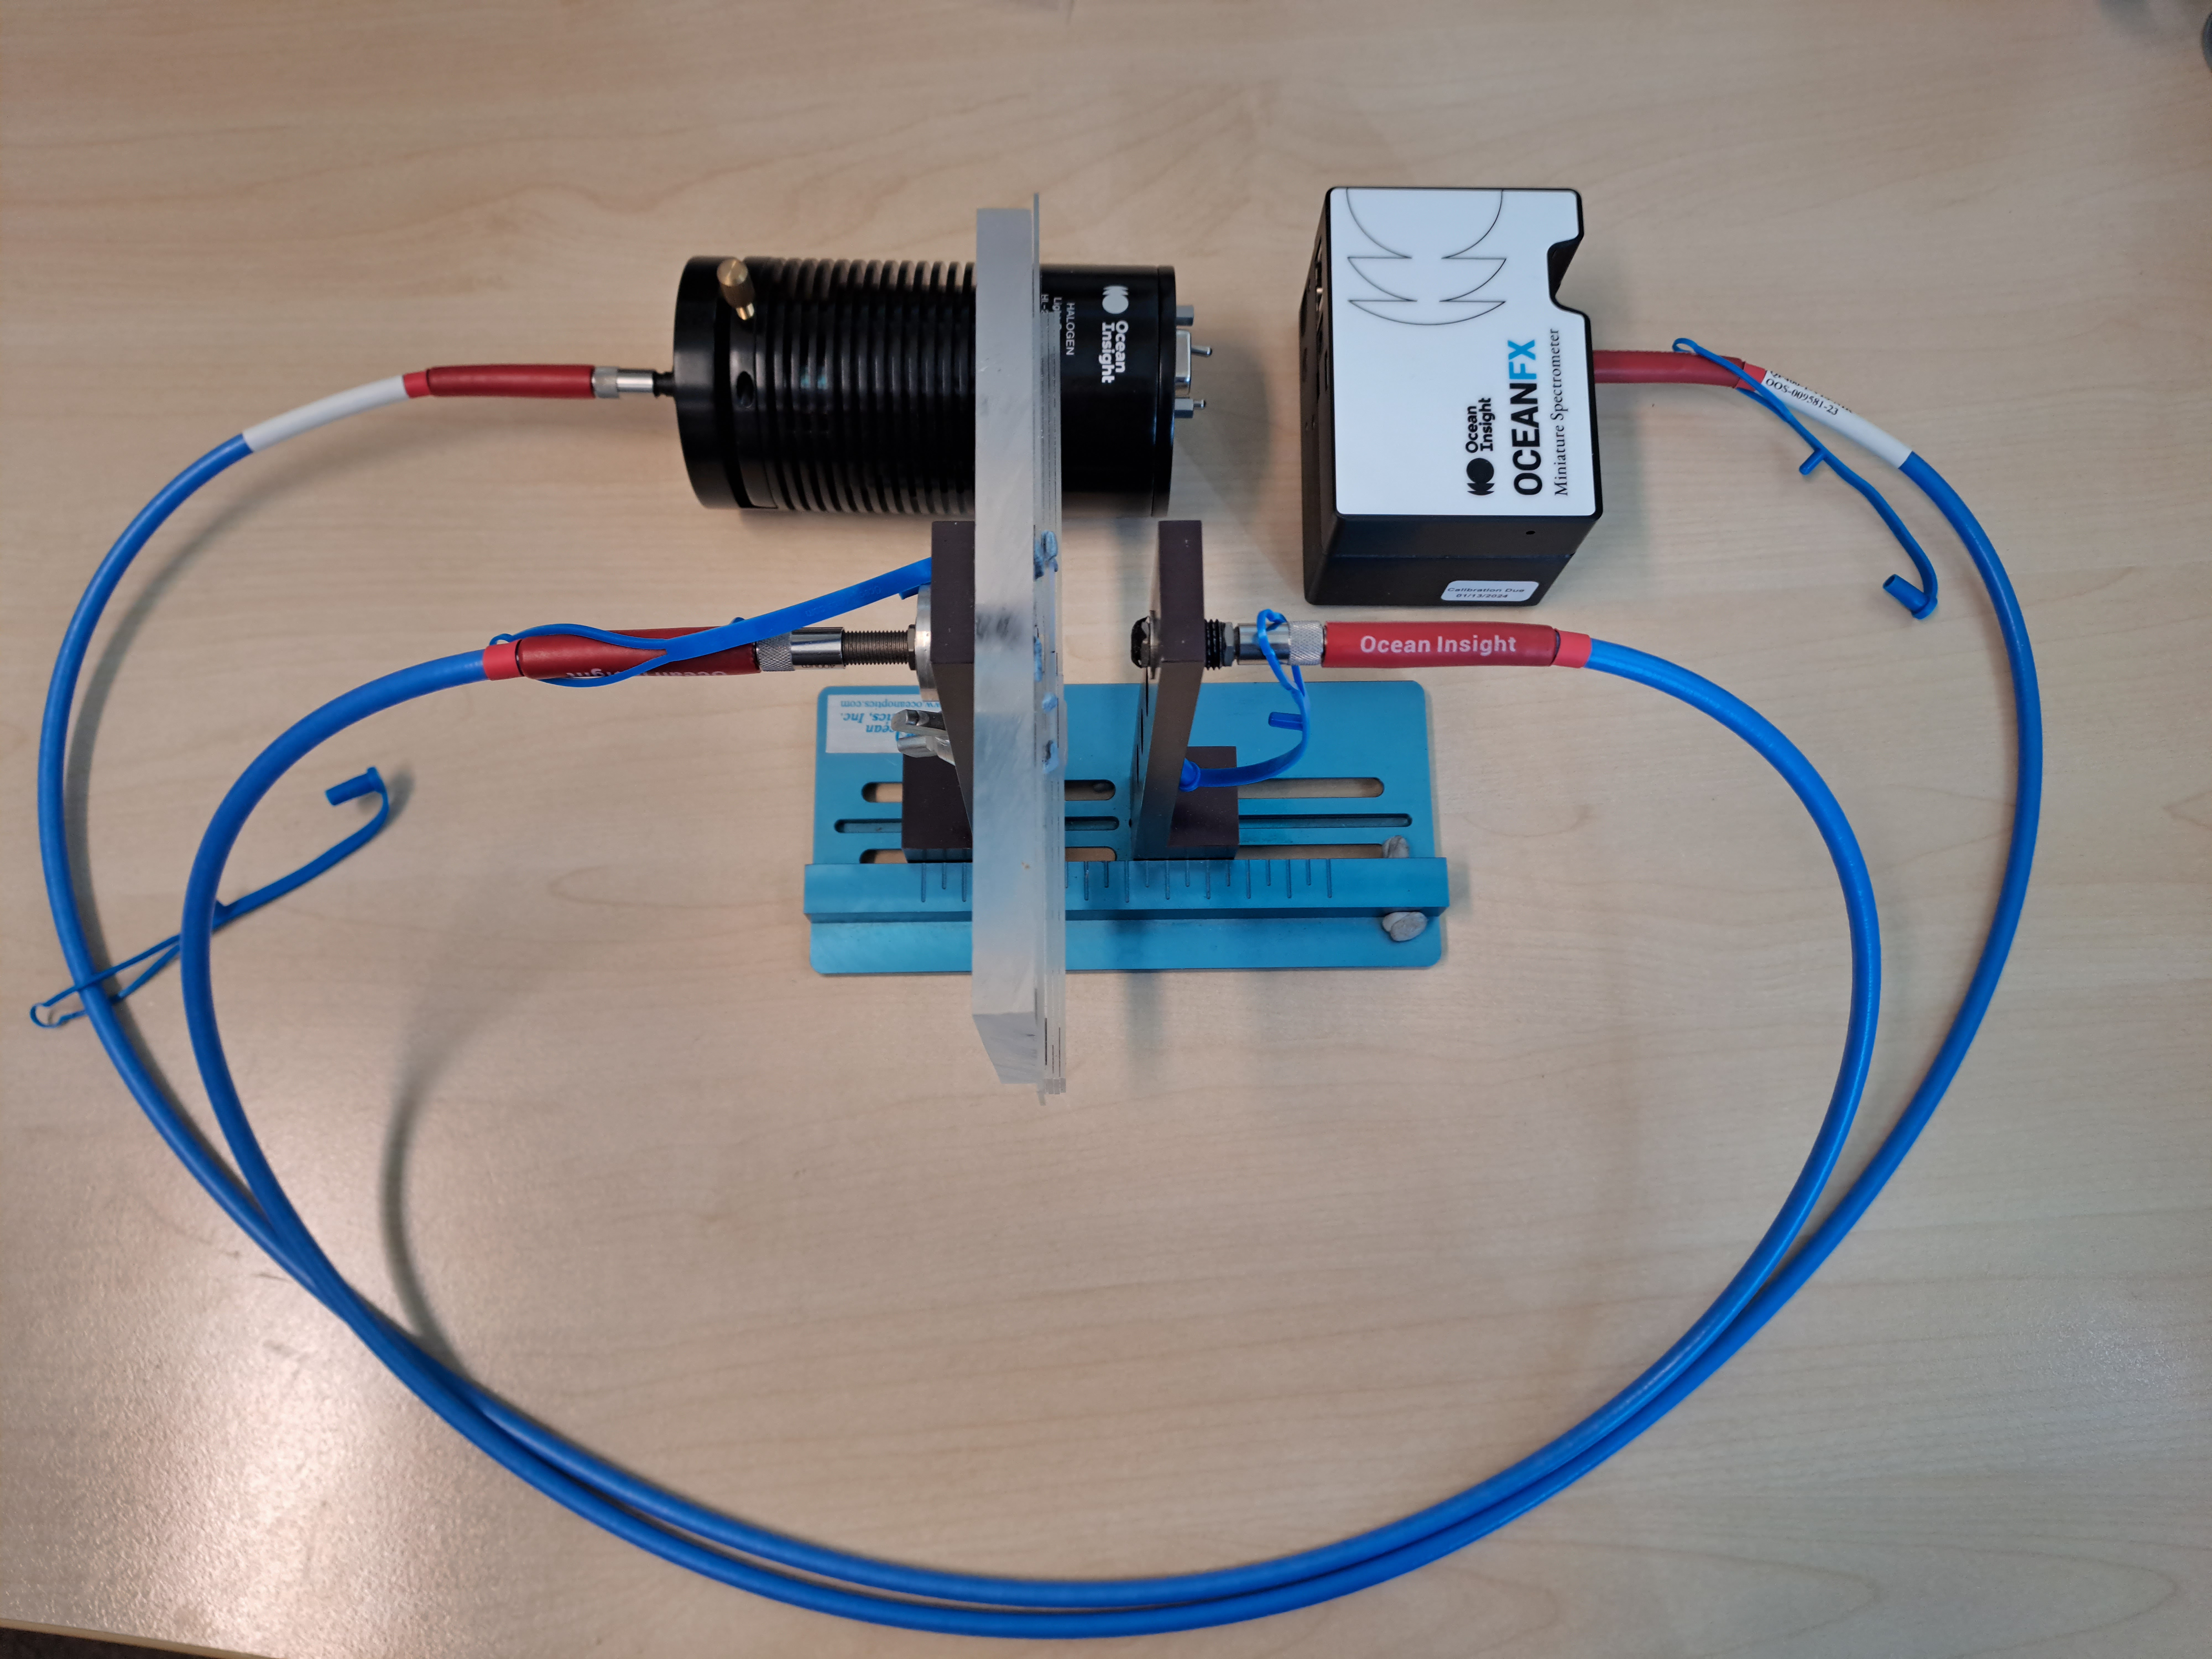
\includegraphics[width=0.6\linewidth]{broadband-test-bed.jpg}
\end{center}
\caption{schematic of the broadband}
\end{figure}
 
\subsection{Program Overview}

\section{Design of Interfacing Microcontroller}
\subsection{Purpose}

The optical monitoring software (for both monochromatic and broadband) must be able to communicate with the Inficon IC-5 deposition controller for two primary reasons: to issue the IC5 with a command to cut deposition, and to inform the OMS software when the deposition has started, so that sample acquisition can begin;
without this ability fully automatic deposition control would not be possible.
In the case of broadband monitoring, the controller must also preform some extra tasks, which will be enumerated later in \ref{intro:design:state_diagram}. Since standard desktops lack GPIO, and are ill suited to tasks where a large amount of time is dedicated to waiting for an event to happen. A micro-controller unit was programmed to provide all the functionality necessary to support both the monochromatic and broadband optical monitoring software. The purpose of combining both sets of requirements into a single unit was to avoid having to reprogram/rewire the circuit when switching between monochromatic and broadband optical monitoring, and provide a single API (on the desktop side) that could be utilised by both the TCP/IP server that communicates with FilmDirector, and by the custom broadband monitoring software. 


\label{intro:design:state_diagram}
\subsection{State Diagram}

\begin{figure}[H]
\begin{center}
\centering
\includegraphics[width=\linewidth]{pico_state_machine.pdf}
\end{center}
\vspace*{-5mm}
\caption{State machine representation of the control flow of the Raspberry Pi Pico micro-controller. In this figure the Serial IO data block represents IO from and to the user; which is used to set the micro-controller into one of the four `active' states/modes (Monochromatic Monitoring, Broadband Monitoring, Monochromatic Observing, Broadband Observing)}
\end{figure}

One of the considerations when designing the program to run the micro-controller was the ability to provide control and functionality to the intellemetrics IL-570 monochromatic optical monitor, as well as the custom broadband optical monitoring system based upon the OceanFX broadband spectrometer. For this reason the micro-controller can be set into one of four `active' states. Each state can be classified using two categories (for $2\times 2$ states). In the broadband modes, the micro-controller triggers the spectrometer when an input trigger to the MCU is received;
the time at which this signal arrives is used to calculate a secondary trigger that captures a reference sample.
This functionality is disabled for the monochromatic modes.
In the monitoring modes, the micro-controller will cut when the user provides a cut command through serial I/O;
If the IC-5 stops depositing before this has been achieved then the program proceeds to an error state.
Conversely, in the observing states, the monitor does not control the deposition,  rather the cut point is solely determined by the IC-5;
if a cut command is received in these states, then the program again proceeds to an error state.

\subsection{Circuit Diagram}

\begin{figure}[H]
\begin{center}
\centering
\includegraphics[width=\linewidth]{KiCad_BBM_Controller.pdf}
\end{center}
\vspace*{-5mm}
\caption{Circuit schematic of the micro-controller and it's connection to the OceanFX spectrometer, the trigger signal, and the Inficon IC-5. The connections to the IC-5 and the trigger signal are opto-isolated, which provides noise filtration (due to low response at higher frequencies) as well as electrical isolation  (up to 4kV) from sources that potentially may experience voltage spikes from EMI or shorts.}
\end{figure}

\chapter{Discussion}
\section{Monochromatic Monitor Performance}
\subsection{Single Layer}
\subsection{Multilayer}
\section{Development of Broadband Optical Monitor}


\end{document}
